\noindent
Initial requirements~:

\noindent
\underline{Meshes}~:\\
Meshes describing the interfaces between regions of homogeneous conductivity. These meshes generally represent:
\begin{itemize}
    \item the inner skull surface
    \item the outer skull surface
    \item the outer scalp surface
\end{itemize}

\noindent
The recommended mesh size is approximately 600 to 800 points per surface.


\medskip

\centerline{
    \hbox{\parbox[t]{5.5cm}{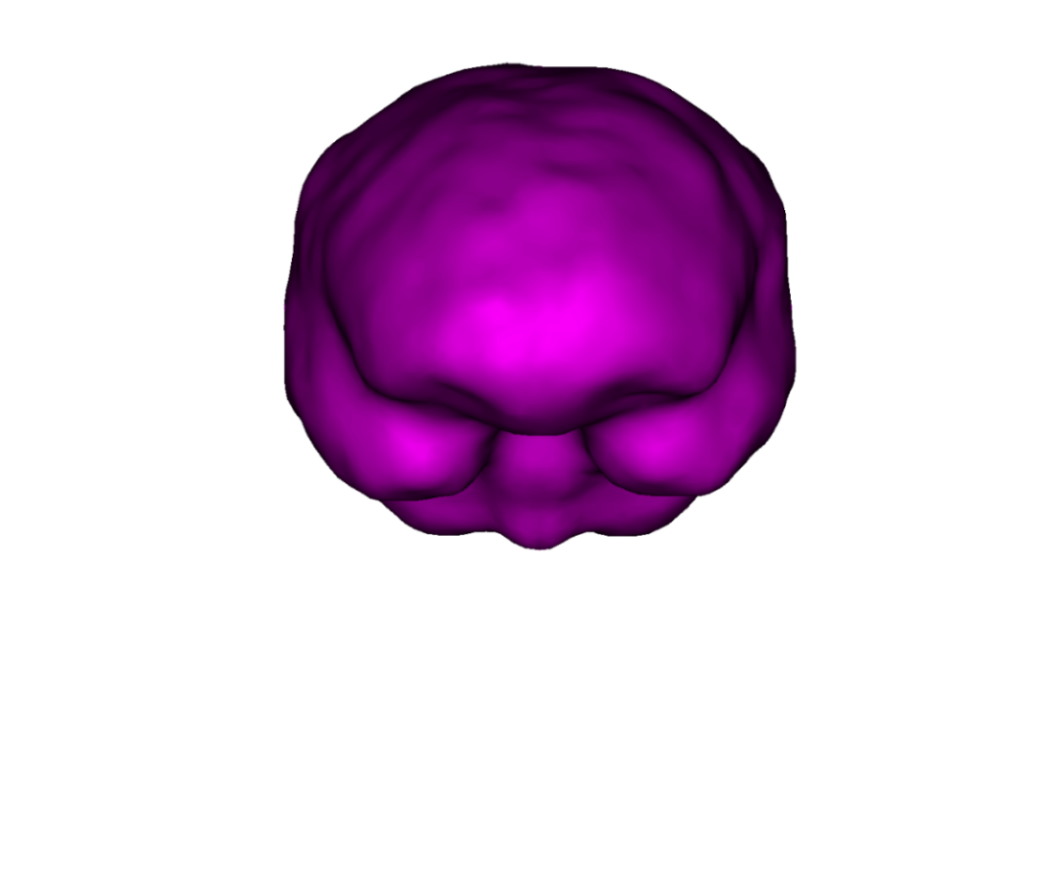
\includegraphics[width=5cm]{tete_couches_brain.png}\\
                            \parbox{5cm}{Surface extérieure au cortex}}
          \parbox[t]{5.5cm}{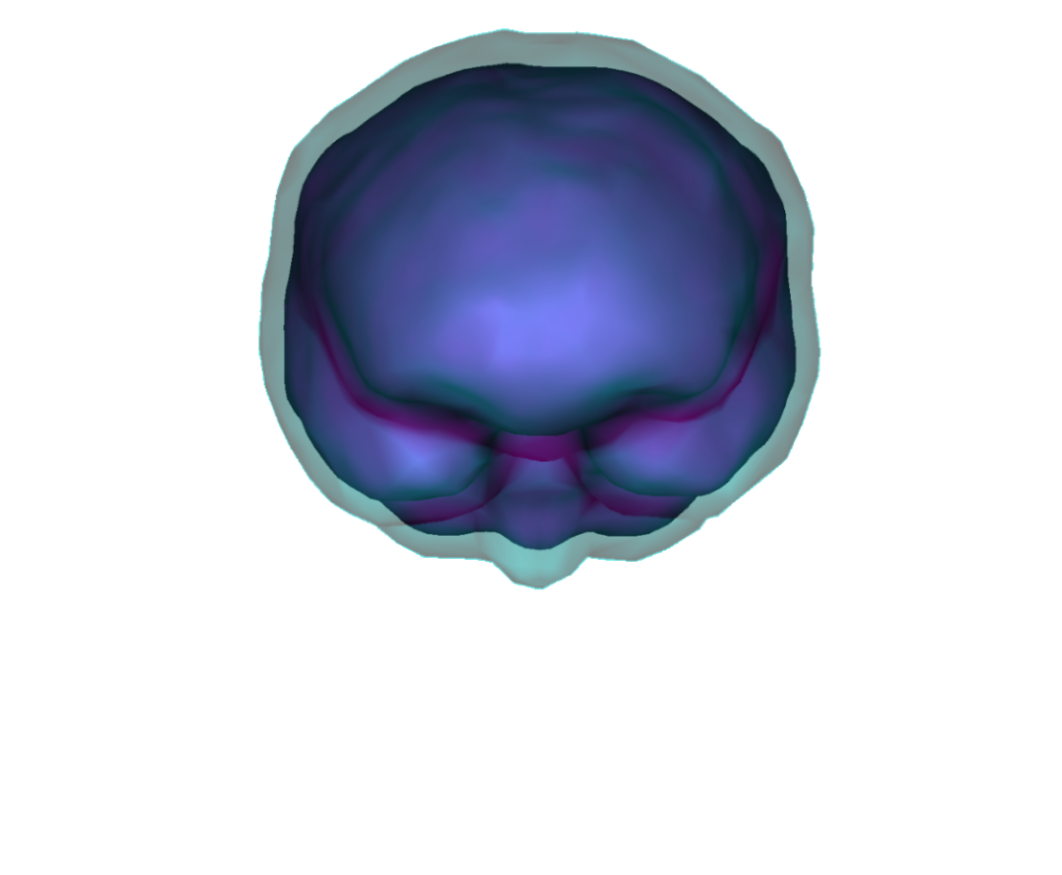
\includegraphics[width=5cm]{tete_couches_brainskull.png}\\\parbox{5cm}{Surface extérieure au crâne en bleu et surface extérieure au cortex en fushia}}
          \parbox[t]{5.5cm}{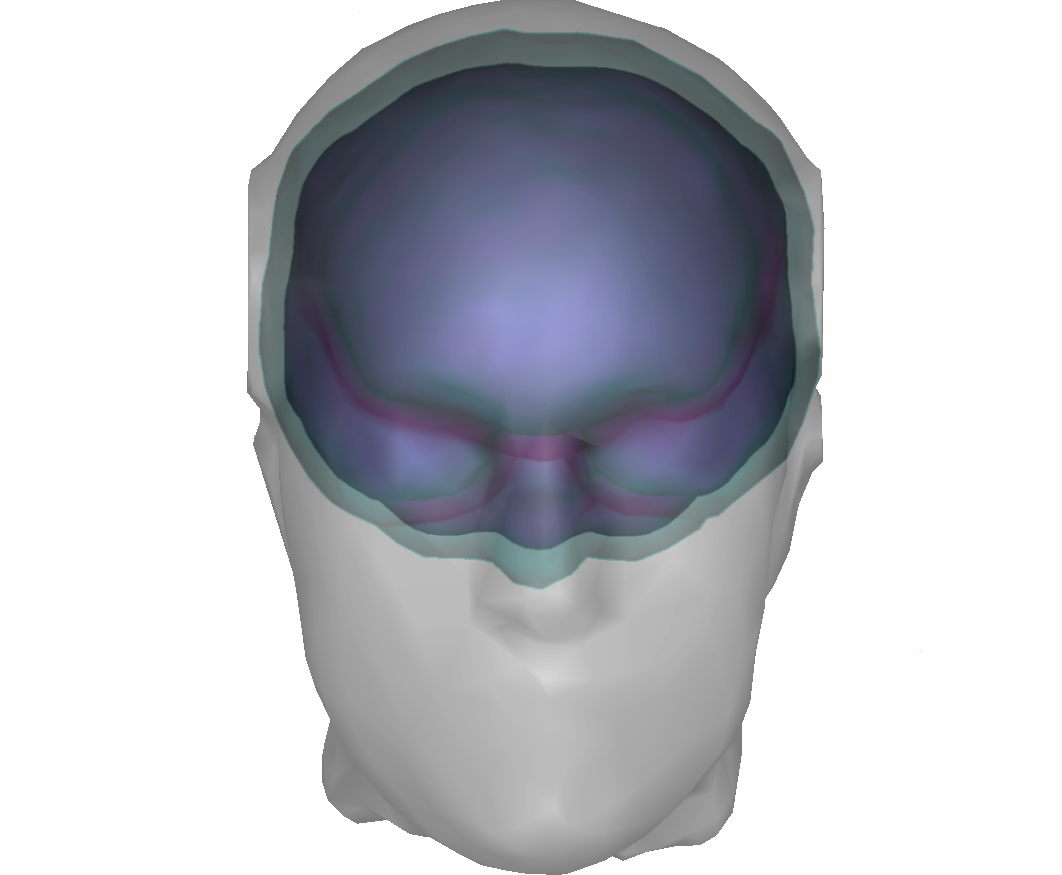
\includegraphics[width=5cm]{tete_couches_brainskullhead.png}\\
                            \parbox{5cm}{Example with three surfaces~:
                                  \begin{itemize}
                                       \item outer scalp (gray)
                                       \item outer skull (blue)
                                       \item inner skull (pink)
                                  \end{itemize}}
                            }
    }
}

\bigskip

\noindent
For distributed sources, a source mesh is required. This is a detailed mesh generally covering the whole cortex. The mesh size should not exceed 35 000 points. 

\begin{center}
    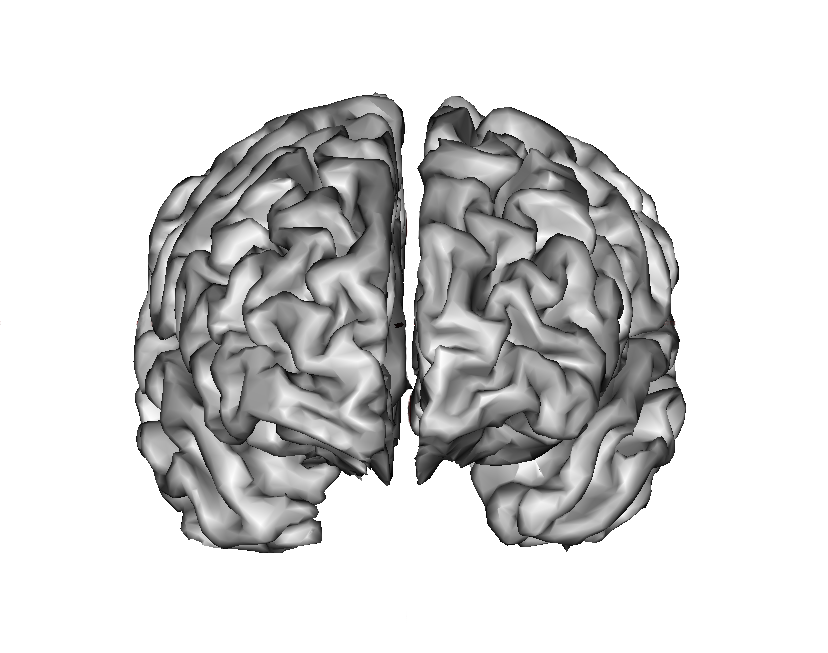
\includegraphics[height=9cm]{cortex.png}\\
Source mesh
\end{center}

\noindent
\underline{Sensors}~:
For EEG, the sensors are defined by the list of the x-y-z coordinates of the electrode positions. The electrodes are considered punctual and are called {\em patches}.	
